\documentclass[letterpaper,11pt]{article}

\usepackage{latexsym}
\usepackage[empty]{fullpage}
\usepackage{titlesec}
\usepackage{marvosym}
\usepackage[usenames,dvipsnames]{color}
\usepackage{verbatim}
\usepackage{enumitem}
\usepackage[hidelinks]{hyperref}
\usepackage{fancyhdr}
\usepackage[english]{babel}
\usepackage{tabularx}
\usepackage{fontawesome5}
\usepackage{multicol}
\setlength{\multicolsep}{-3.0pt}
\setlength{\columnsep}{-1pt}
\input{glyphtounicode}

%new packages

\usepackage{fontenc}
\usepackage{amsmath}
\usepackage{amssymb}
\usepackage{graphicx}



%----------FONT OPTIONS----------

\pagestyle{fancy}
\fancyhf{} % clear all header and footer fields
\fancyfoot{}
\renewcommand{\headrulewidth}{0pt}
\renewcommand{\footrulewidth}{0pt}

% Adjust margins
\addtolength{\oddsidemargin}{-0.6in}
\addtolength{\evensidemargin}{-0.5in}
\addtolength{\textwidth}{1.19in}
\addtolength{\topmargin}{-.7in}
\addtolength{\textheight}{1.4in}

\urlstyle{same}

\raggedbottom
\raggedright
\setlength{\tabcolsep}{0in}

% Sections formatting
\titleformat{\section}{
  \vspace{-4pt}\scshape\raggedright\large\bfseries
}{}{0em}{}[\color{black}\titlerule \vspace{-5pt}]



% Ensure that generate pdf is machine readable/ATS parsable
\pdfgentounicode=1

%-------------------------
% Custom commands
\newcommand{\resumeItem}[1]{
  \item\small{
    {#1 \vspace{-2pt}}
  }
}

\newcommand{\classesList}[4]{
    \item\small{
        {#1 #2 #3 #4 \vspace{-2pt}}
  }
}

\newcommand{\resumeSubheading}[4]{
  \vspace{-2pt}\item
    \begin{tabular*}{1.0\textwidth}[t]{l@{\extracolsep{\fill}}r}
      \textbf{#1} & \textbf{\small #2} \\
      \textit{\small#3} & \textit{\small #4} \\
    \end{tabular*}\vspace{-7pt}
}

\newcommand{\resumeSubSubheading}[2]{
    \item
    \begin{tabular*}{0.97\textwidth}{l@{\extracolsep{\fill}}r}
      \textit{\small#1} & \textit{\small #2} \\
    \end{tabular*}\vspace{-7pt}
}

\newcommand{\resumeProjectHeading}[2]{
    \item
    \begin{tabular*}{1.001\textwidth}{l@{\extracolsep{\fill}}r}
      \small#1 & \textbf{\small #2}\\
    \end{tabular*}\vspace{-7pt}
}


\newcommand{\resumeSubItem}[1]{\resumeItem{#1}\vspace{-4pt}}

\renewcommand\labelitemi{$\vcenter{\hbox{\tiny$\bullet$}}$}
\renewcommand\labelitemii{$\vcenter{\hbox{\tiny$\bullet$}}$}

\newcommand{\resumeSubHeadingListStart}{\begin{itemize}[leftmargin=0.0in, label={}]}
\newcommand{\resumeSubHeadingListEnd}{\end{itemize}}
\newcommand{\resumeItemListStart}{\begin{itemize}}
\newcommand{\resumeItemListEnd}{\end{itemize}\vspace{-5pt}}

\begin{document}
\fontfamily{cmr}\selectfont
\begin{center}
\parbox{3.0cm}{%
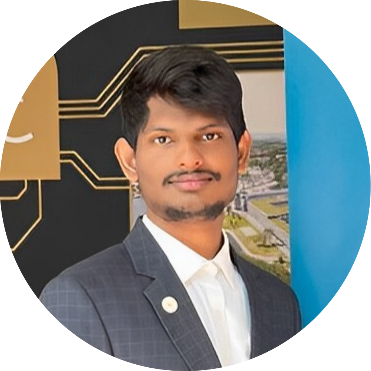
\includegraphics[width=2.7cm,clip]{images/resume_pic_m.png}}
}
\parbox{\dimexpr\linewidth-3.8cm\relax}{
\vspace{-20pt}
\begin{tabularx}{\linewidth}{L r} \\
    {\Huge \scshape  Venkata Sai Yakkshit Reddy Asodi}~
    \href{https://www.cedzlabs.com/yakkshit}{\vspace{1pt}}\\
      Berlin, Germany. \\ \vspace{1pt}
     \small \raisebox{-0.1\height}\faPhone\ +91 8179936156 ~ \href{mailto:saiyakkshit2001@gmail.com}{\raisebox{-0.2\height}\faEnvelope\  {saiyakkshit2001@gmail.com}} ~ 
    \href{https://linkedin.com/in/yakkshit/}{\raisebox{-0.2\height}\faLinkedin\ {yakkshit}}  ~
    \href{https://yakkshit.com/}{\raisebox{-0.2\height}\faGlobe\ {yakkshit.com}}  ~
    \href{https://github.com/yakkshit}{\raisebox{-0.2\height}\faGithub{ yakkshit}}
    \vspace{-8pt}
\end{tabularx}
}
\end{center}

\vspace{-23pt}
\section{Summary \faLink}
Passionate Junior Developer with strong Python and AI experience, seeking to leverage my technical skills and business acumen as a Technical Founder Associate at Cuinti. Demonstrated ability in building conversational AI systems and developing full-stack applications. Strong track record of quickly learning new technologies and translating business requirements into technical solutions. Eager to contribute to Cuinti's mission of revolutionizing sales training through AI-powered solutions.

\section{\href{https://www.linkedin.com/in/yakkshit/details/skills/}{Technical Skills} \faLink}
\begin{itemize}[leftmargin=0.15in, label={}]
\small{\item{
\textbf{Languages - }{Python, JavaScript (ES6+), HTML5, CSS3} \\
\textbf{Technologies - }{Docker, MongoDB, Redis, RESTful APIs, Git} \\
\textbf{AI/ML - }{HuggingFace, LLMs, Conversational AI, Azure AI} \\
\textbf{Frontend - }{React, Vue.js, Responsive Design} \\
}}
\end{itemize}
\vspace{-10pt}

\section{Experience \faLinkedin}
\resumeSubHeadingListStart

\resumeSubheading
{\large Circleup AG \faBuilding}{December 2023 -- July 2024}
{Full Stack Engineer (AI Focus)}{\faMapMarker \hspace{0.1cm} Zurich, Switzerland}\\
\vspace{10pt}
\textbf{Responsibilities:}
\resumeItemListStart
\vspace{-10pt}
\resumeItem{Developed and deployed conversational AI systems using Python and HuggingFace, improving customer interaction accuracy by 40\%. Implemented Docker containerization for streamlined deployment.}
\resumeItem{Collaborated with product teams to translate business requirements into technical solutions, leading to successful implementation of 3 major features that increased user engagement by 25\%.}
\resumeItemListEnd
\vspace{-3pt}
\textbf{Environment:}\emph{Python, Docker, MongoDB, HuggingFace, RESTful APIs, Agile}

\resumeSubheading
{Cedzlabs \faBuilding}{March 2023 -- July 2024}
{Junior Developer}{\faMapMarker \hspace{0.1cm} Remote}\\
\vspace{10pt}
\textbf{Responsibilities:}
\vspace{-10pt}
\resumeItemListStart
\resumeItem{Built and maintained Python microservices for processing audio data, implementing efficient data compression techniques that reduced storage costs by 30\%.}
\resumeItem{Developed automated testing frameworks that reduced QA time by 50\% while maintaining 99\% test coverage.}
\resumeItemListEnd
\vspace{-3pt}
\textbf{Environment:}\emph{Python, Redis, Docker, Audio Processing, Git}

\section{Projects \faGithub}
\vspace{-5pt}
\resumeSubHeadingListStart
\resumeProjectHeading
{\textbf{\href{https://github.com/yakkshit/sales-coach-ai}{SalesCoach AI}} $|$ \emph{Python, HuggingFace, Azure}}{January 2024}\\
\vspace{6pt}
\textbf{Description:}
\vspace{-5pt}
\resumeItemListStart
\resumeItem{Developed an AI-powered sales coaching platform that provides real-time feedback on sales conversations. Implemented custom fine-tuning of language models for sales-specific dialogue, achieving 85\% accuracy in feedback generation. Integrated with Twilio for voice processing and Azure for scalable deployment.}
\resumeItemListEnd
\vspace{4pt}
\textbf{Tools:}\emph{Python, HuggingFace, Azure, Twilio, MongoDB}
\vspace{-10pt}

\resumeProjectHeading
{\href{https://github.com/yakkshit/audio-analytics}{\textbf{Audio Analytics Platform}} $|$ \emph{Python, Docker}}{November 2023}\\
\vspace{6pt}
\textbf{Description:}
\vspace{-5pt}
\resumeItemListStart
\resumeItem{Created a system for processing and analyzing audio conversations using Python and μ-law compression. Implemented real-time processing pipeline with Redis for caching and MongoDB for storage. Achieved 40\% reduction in processing time through optimization.}
\resumeItemListEnd
\vspace{4pt}
\textbf{Tools:}\emph{Python, Docker, Redis, MongoDB, Audio Processing}
\vspace{-12pt}

\section{Achievements / Extracurricular}
\resumeSubHeadingListStart
\resumeItemListStart
\resumeItem{Led a team of 3 developers in implementing Agile methodologies, resulting in 30\% faster project delivery.}
\resumeItem{Contributed to open-source conversational AI projects on GitHub, with 100+ stars and 20+ forks.}
\resumeItem{Awarded "Best Technical Innovation" at European AI Hackathon 2023 for developing an AI-powered sales training solution.}
\resumeItemListEnd

\resumeSubHeadingListEnd
\textbf{Strengths:}\emph{Fast learner, problem-solver, excellent communicator, business-minded} \\
\textbf{Languages:}\emph{Telugu - Native $|$ English - Fluent $|$ Hindi - Fluent $|$ German - Elementary $|$ Swedish - Elementary}

\vspace{10pt}
\end{document}